\providecommand{\main}{../../../..}
\documentclass[\main/dresen_thesis.tex]{subfiles}
\renewcommand{\thisPath}{\main/chapters/theoreticalBackground/scattering/gisas}
\begin{document}
  \subsection{Grazing Incidence Small-Angle Scattering}\label{sec:theoreticalBackground:scattering:GISAS}
    Additionally to the vertical structure, it is interesting to study the lateral structure of an ensemble of nanoparticles to obtain the complete three dimensional information.
    For this purpose grazing-incidence small-angle scattering (GISAS) has proven an efficient technique to measure the off-specular scattering from which in-plane order within a sample can be extracted with high resolution \cite{Renaud_2009_Probi}.

    In GISAS, the incident angle is chosen to be close to the critical angle of the sample, where the Born approximation is not accurate enough to reliably calculate the scattering.
    It has to be modified to account for reflection and refraction effects at the interfaces of a sample.
    This is provided by the the distorted-wave Born approximation (DWBA), where the scattering wave function is no longer assumed to be a plane wave within the sample such as in the Born approximation.
    For the DWBA, the scattering potential is assumed to be decomposable in
    \begin{align}
      V(\vec{r}) \eq \bar{V}(\vec{r}) + \delta V(\vec{r}).
    \end{align}
    Where the potential $\bar{V}(\vec{r})$ can be treated exactly to determine the wave function of the scattering problem for the case $\delta V(\vec{r})\eq 0$.
    And the small perturbation $\delta V \ll \bar{V}$ is treated analogue to the Born approximation, but instead of plane waves, the previously determined wave function is used.
    In GISAS, $\bar{V}$ represents the one dimensional description of the layered structure for the sample, and $\delta V$ is the in-plane fluctuations \textit{e.g.} due to nanoparticles in a layer.
    By using a transfer matrix ansatz for the layered structure, it is straight forward to calculate the incoming and outgoing amplitudes of the wave function in each layer.
    Then the modulation of the scattered intensity due to $\delta V$ is essentially given by the Fourier transform of $\delta V$ summed for each layer and weighted with the incoming and outgoing amplitude.

    \begin{figure}
      \centering
      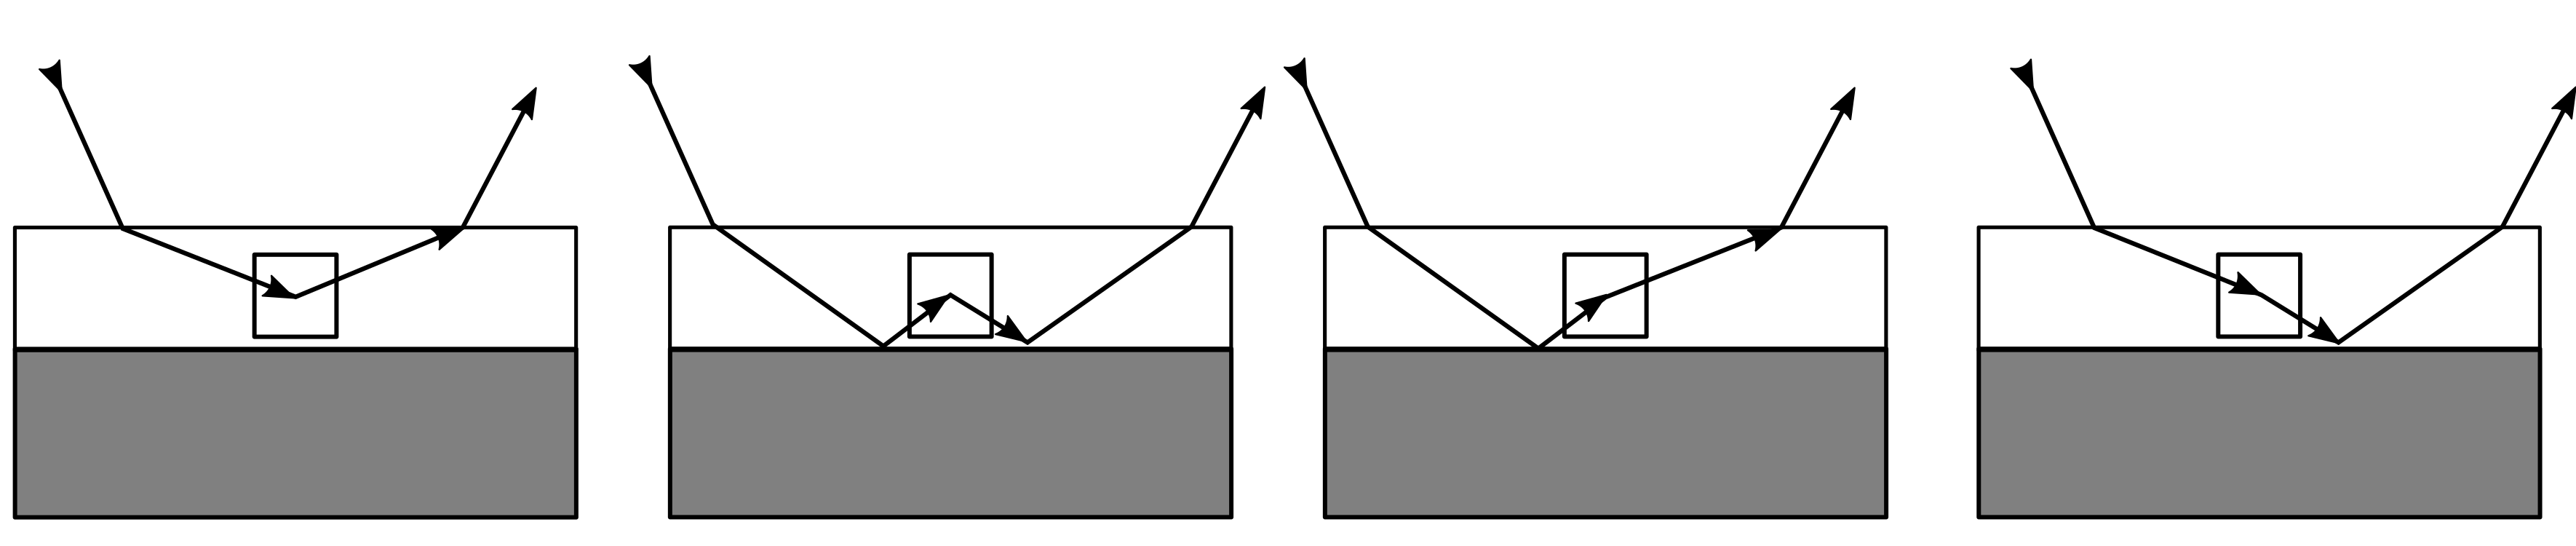
\includegraphics{scatteringTheory_gisaxs_multiple_paths}
      \caption{\label{fig:theoreticalBackground:scattering:gisas:multiplePaths}Possible scattering processes that can occur for a fixed incident and outgoing angle, when reflection and refraction are accounted for by the DWBA.}
    \end{figure}
    Care has to be taken whether the scattering process with $\delta V$ happens for a wave moving up or downward in the sample in the layer, and whether it results in an upward or downward moving wave.
    The incoming and outgoing angle are determined by the source and detector position for the calculation.
    As all reflections processes on the layer interfaces are accounted for in the DWBA, four paths are possible for a single scattering event on $\delta V$ in a layer to contribute.
    These four possible combinations, depicted in \reffig{fig:theoreticalBackground:scattering:gisas:multiplePaths}, have to be considered when calculating the scattering amplitude, where the scattering vector for each combination of upward and downward moving waves has to be calculated and used in the Fourier transform accordingly.

    The detailed implementation of the DWBA for nanostructures is well discussed in \cite{Lazzari_2002_Isgis}, as well as more recently in the manual of the software package BornAgain \cite{Burle_2018_borna}, which is used for the simulation of GISAS data in this work.
    As in the case of reflectometry, it is possible to obtain information about the electron density using GISAS with X-rays (GISAXS), and about the nuclear and magnetic structure using (polarized) neutrons (GISANS, polGISANS).
    The experimental details for the data acquisition and treatment are discussed in \refapp{app:methods:gisaxs} and \refapp{app:methods:gisans} respectively.
\end{document}